%------------------------------------------------------------------------------
% Author(s):
% Varaun Ramgoolie
% Copyright:
%  Copyright (C) 2020 Brad Bachu, Arjun Mohammed, Varaun Ramgoolie, Nicholas Sammy
%
%  This file is part of Applied-Mathematics-Unit2 and is distributed under the
%  terms of the MIT License. See the LICENSE file for details.
%
%  Description:
%     Linear Programming graph for 2016 q2
%------------------------------------------------------------------------------

\documentclass[crop,tikz]{standalone}
\usepackage{pgfplots}
\usepackage{../../../../src/tikzappmath}
\usetikzlibrary{patterns}

\begin{document}
	
	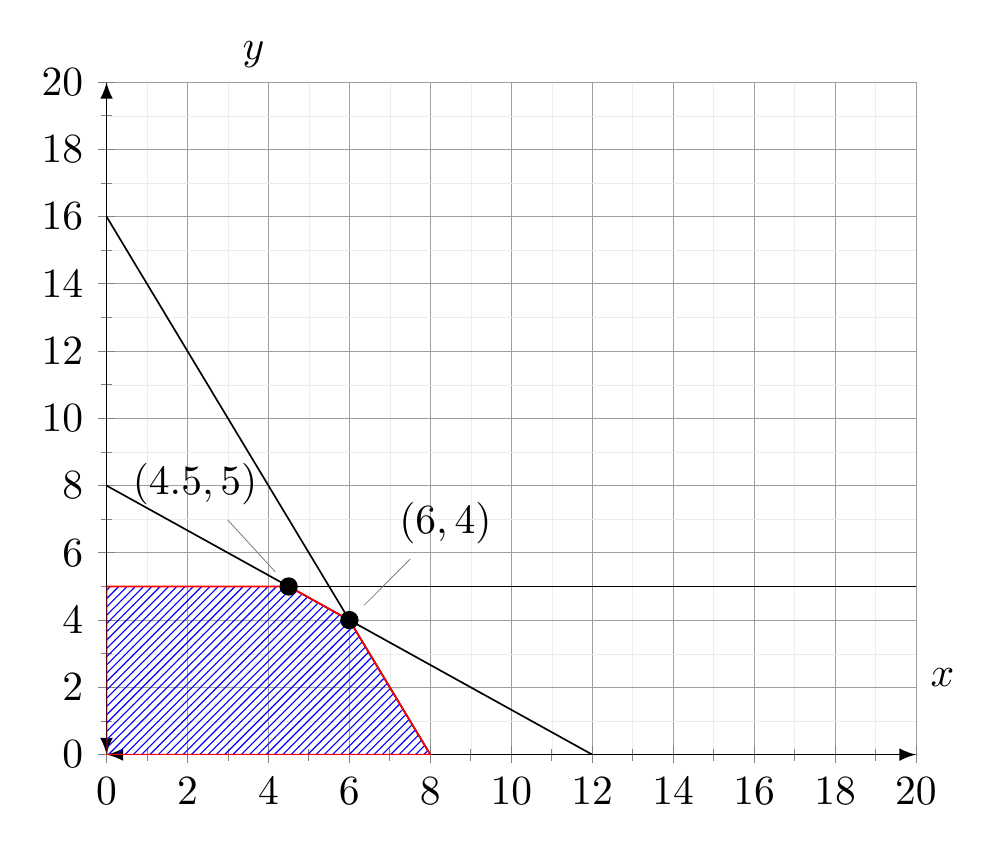
\begin{tikzpicture}[scale=1.5]
		\begin{axis}
			[
			xmin=-0,xmax=20,
			ymin=0,ymax=20,
			grid=both,
			grid style={line width=.1pt, draw=darkgray!10},
			major grid style={line width=.2pt,draw=darkgray!50},
			axis lines=left,
			minor tick num=1,
			enlargelimits={abs=0},
			axis line style={latex-latex},
			samples=100,
			domain = -20:20,
			ytick={0,2,4,...,20},
			xtick={0,2,4,...,20},
			xlabel={$x$},
			ylabel={$y$},
			x label style={at={(axis description cs:1,0.15)},anchor=north west},
			y label style={at={(axis description cs:0.15,1)},anchor=south west, rotate=-90}
			]
			
			\addplot [mark=dot] coordinates{(12,0)  (0,8)};
			
			\addplot [mark=dot] coordinates {(8,0) (0,16)};
			
			\addplot [mark=dot] coordinates {(0,5) (100,5)};
			
			\addplot [red,pattern=north east lines,pattern color=blue] coordinates {(0,5) (4.5,5) (6, 4) (8,0)} \closedcycle;	
			
			\node [pin=104:{$(4.5,5)$}] at (axis cs:4.5,5) {};
			
			\addplot [mark=*] coordinates{(4.5, 5)};
			
			\node [pin=60:{$(6,4)$}] at (axis cs:6,4) {};
			
			\addplot [mark=*] coordinates{(6,4)};
			
		\end{axis}
	\end{tikzpicture}
	
\end{document}